\chapter{Bedienungsanleitung}

    \section{Öffnen des Projektes}
        Zunächst wird \textit{Quartus Prime Lite} gestartet.
        Sobald das Hauptfenster geöffnet wurde kann über den Menüpunkt \textit{File}
        der Untermenüpunkt \textit{Open Project}, wie in Abbildung \ref{fig:quartus_open_project} gezeigt,
        geklickt werden. Daraufhin öffnet sich ein Dateibrowser (Abbildung \ref{fig:quartus_select_project})
        durch den das Projekt ausgewählt werden kann.
        Der relative Pfad des Projektes im Repository ist dabei \textit{RiscV-i32/CPU/Design/RiscV.qpf}
        
        \begin{figure}[H]
            \centering
            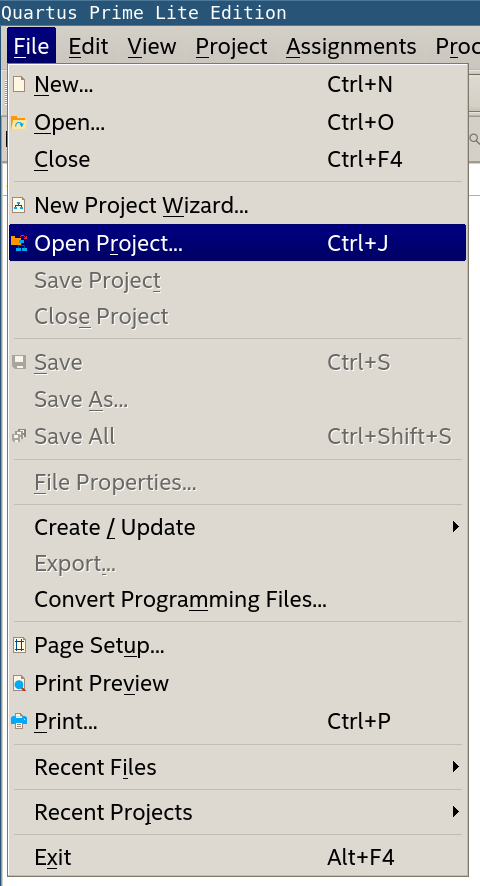
\includegraphics[scale=0.6]{img/quartus_open_project.png}
            \caption{Öffnen des Projektes in Quartus}
            \label{fig:quartus_open_project}
        \end{figure}

        \begin{figure}[H]
            \centering
            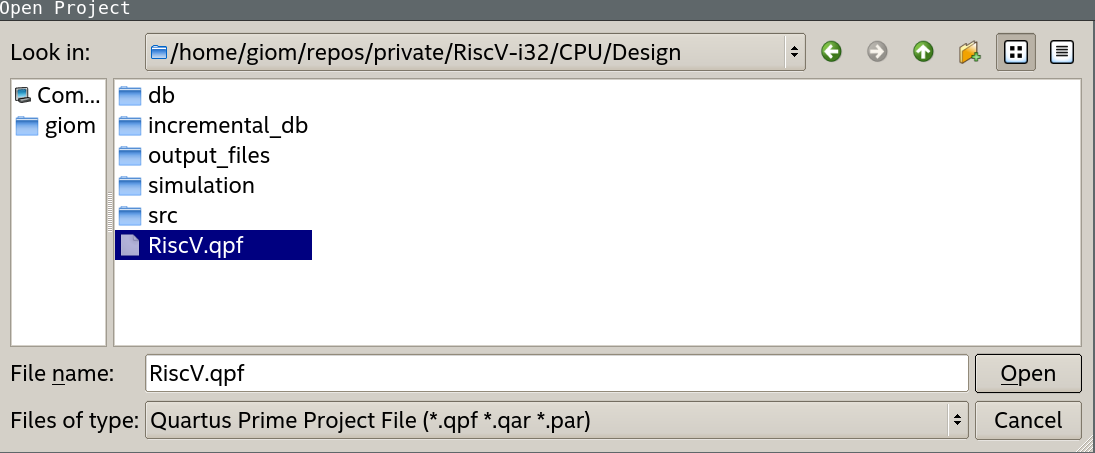
\includegraphics[scale=0.6]{img/quartus_select_project.png}
            \caption{Öffnen des Projektes in Quartus}
            \label{fig:quartus_select_project}
        \end{figure}


    \section{Bauen des Projektes}
        Sobald sich das Projekt erfolgreich geöffnet hat, kann das Bauen über einen Klick
        auf das \textit{Play}-Symbol (Abbildung \ref{fig:quartus_play}) gestartet werden. Das eigentliche Bauen kann, je nach
        Leistung des Rechners mehrere Minuten dauern. Dabei wird der Status im unteren
        Fensterdrittel angezeigt. War das Bauen erfolgreich wird die Meldung
        \textit{Quartus Prime Full Compilation was successful} (Abbildung \ref{fig:quartus_build_sucessful})
        angezeigt.

        \begin{figure}[H]
            \centering
            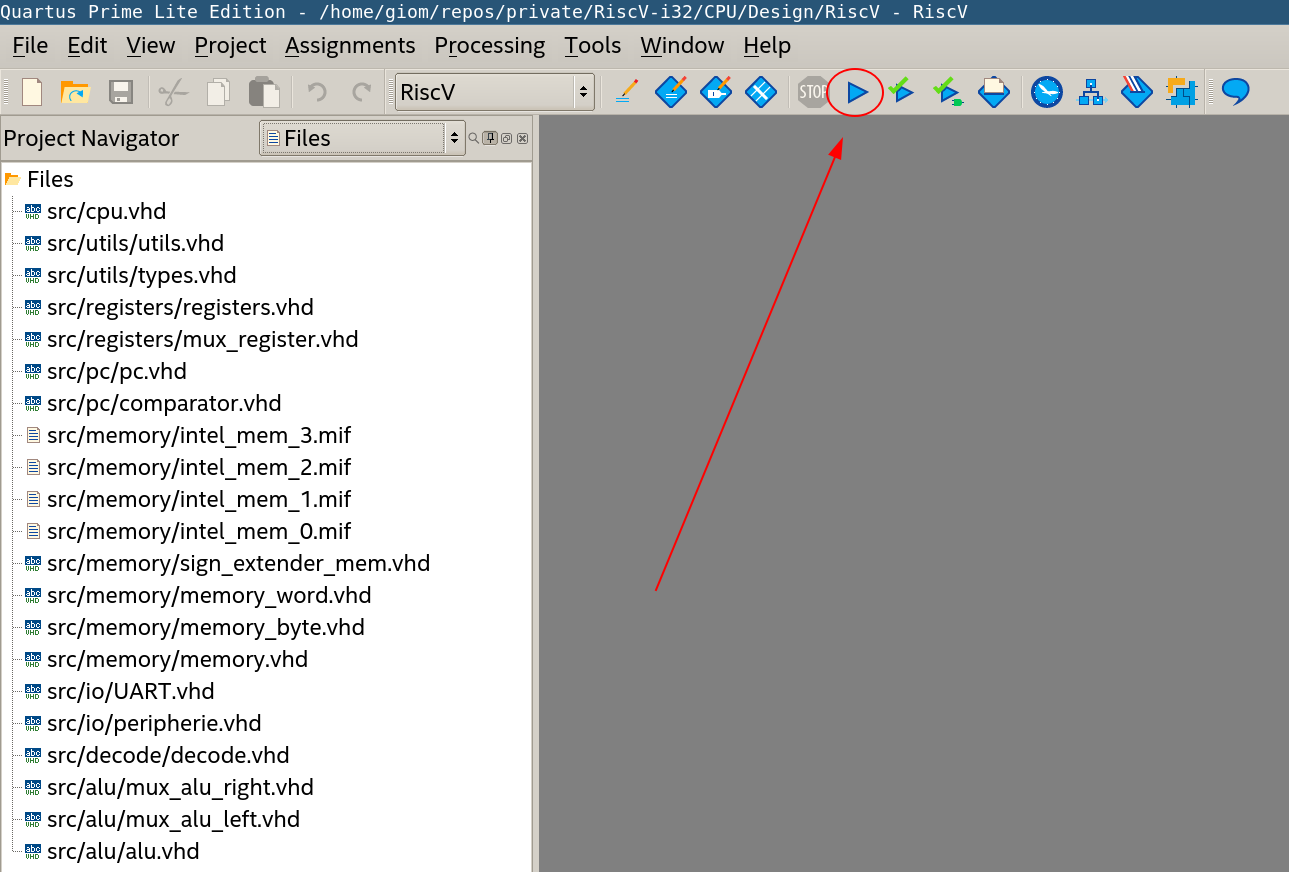
\includegraphics[scale=0.6]{img/quartus_build.png}
            \caption{Bauen des Projektes in Quartus}
            \label{fig:quartus_play}
        \end{figure}

        \begin{figure}[H]
            \centering
            
\includegraphics[scale=0.6]{img/quartus_build_sucessfull.png}
            \caption{Erfolgreiches Bauen des Projektes in Quartus}
            \label{fig:quartus_build_sucessful}
        \end{figure}


    \section{Flashen des FPGAs}

    Zunächst muss das FPGA-Board über USB angeschlossen werden. Zusätzlich muss der Treiber schon installiert sein.
    Ist dies der Fall kann über den Menüpunkt \textit{Tools} der Untermenüpunkt \textit{Programmer}
    ausgewählt werden. (Abbildung \ref{fig:quartus_programmer})
    Dadurch öffnet sich der Programmer (Abbildung \ref{fig:quartus_programmer_window})
    und die Hardware kann durch einen Klick auf \textit{Hardware Setup} eingerichtet werden.
    Ein weiteres Fenster öffnet sich (Abbildung \ref{fig:quartus_programmer_select_hardware}).
    Ein Doppelklick auf \textit{Arrow-USB-Blaster (1)} wählt das FPGA-Board als Ziel für den Programmer.
    Dies kann durch \textit{Currently selected Hardware (2)} bestätigt werden. Ein weiterer Klick 
    \textit{close} schließt das Fenster wieder. Nun kann über \textit{Start}
    (Abbildung \ref{fig:quartus_programmer_start}) das eigentliche Flashen beginnen.
    Eine visuelles Rückmeldung bietet hierbei der Ladebalken \textit{Progress}.
    

    \begin{figure}[H]
        \centering
        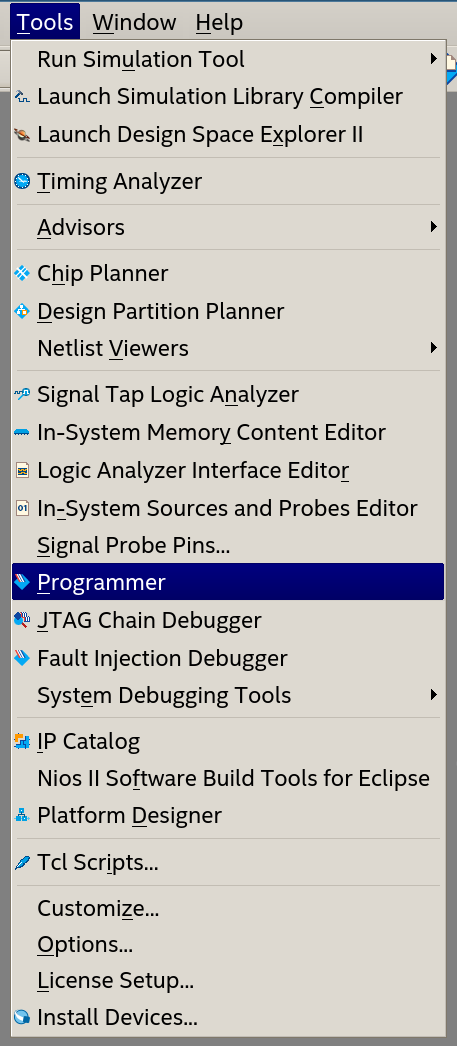
\includegraphics[scale=0.6]{img/quartus_programmer.png}
        \caption{Öffnen des Programmers in Quartus}
        \label{fig:quartus_programmer}
    \end{figure}

    \begin{figure}[H]
        \centering
        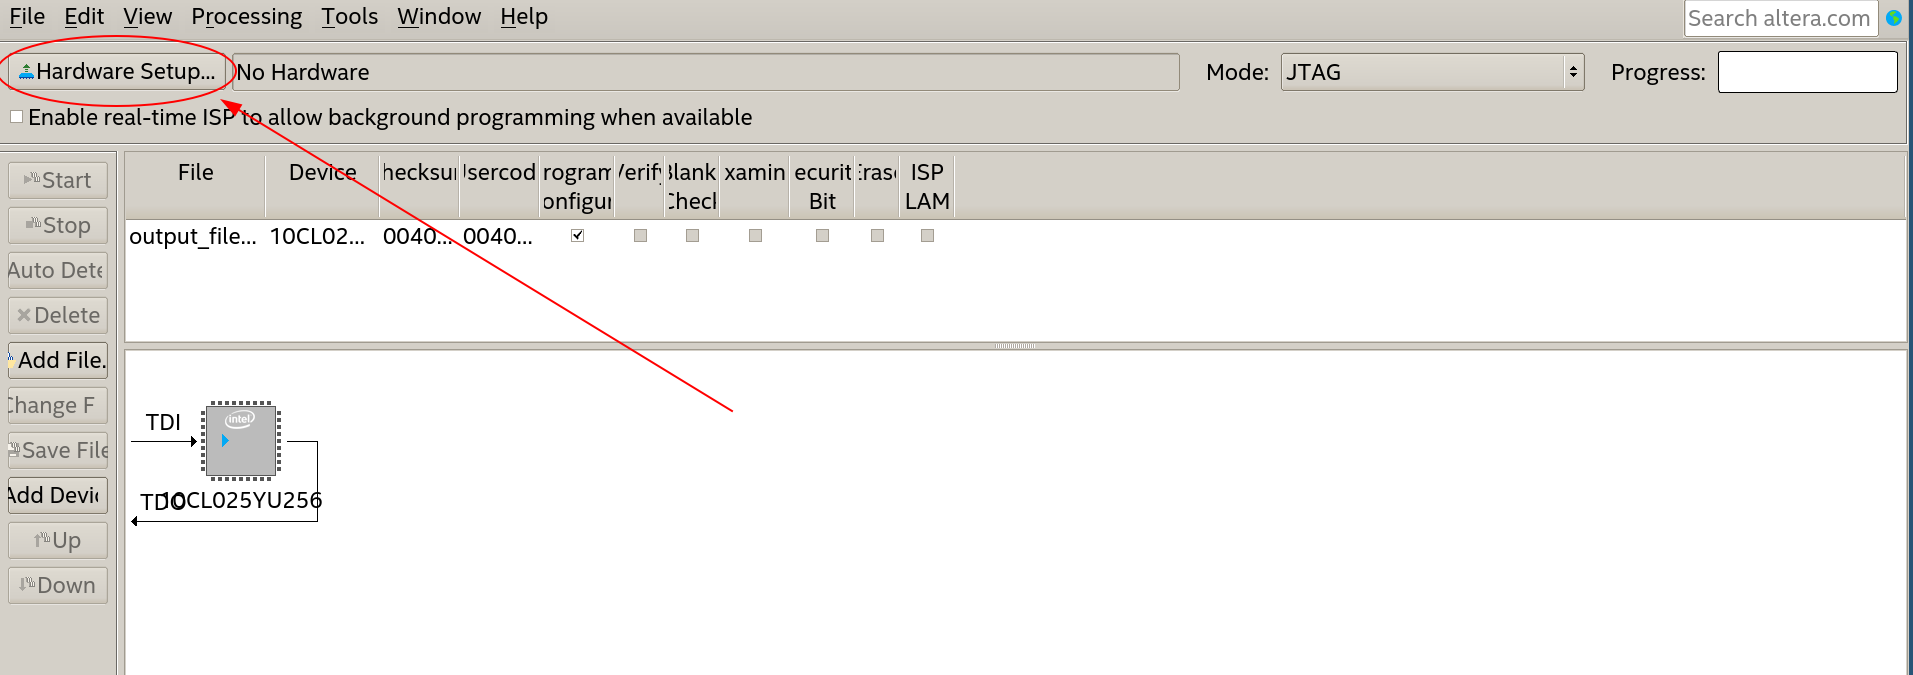
\includegraphics[scale=0.6]{img/quartus_programmer_select_hardware.png}
        \caption{Einrichten der Hardware in Quartus}
        \label{fig:quartus_programmer_window}
    \end{figure}

    \begin{figure}[H]
        \centering
        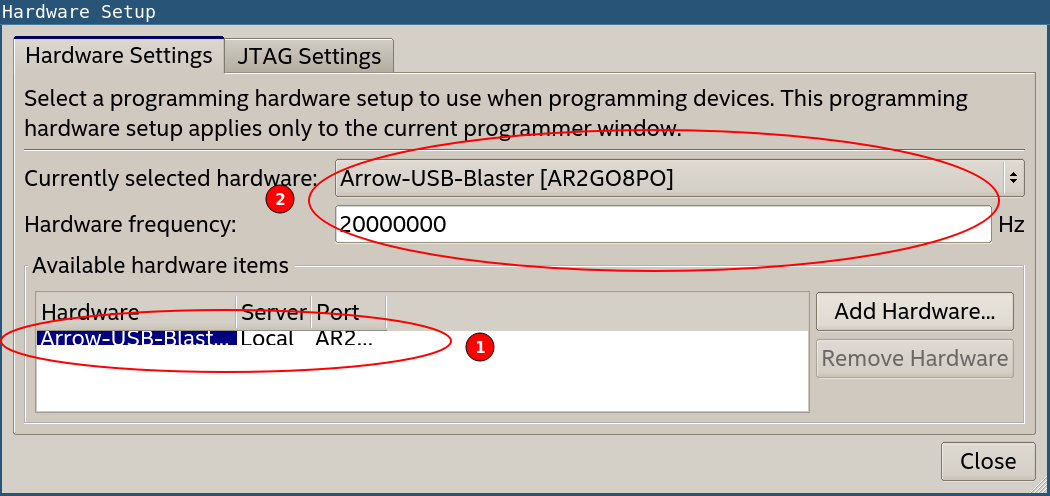
\includegraphics[scale=0.6]{img/quartus_programmer_select_hardware2.png}
        \caption{Einrichten der Hardware in Quartus}
        \label{fig:quartus_programmer_select_hardware}
    \end{figure}

    \begin{figure}[H]
        \centering
        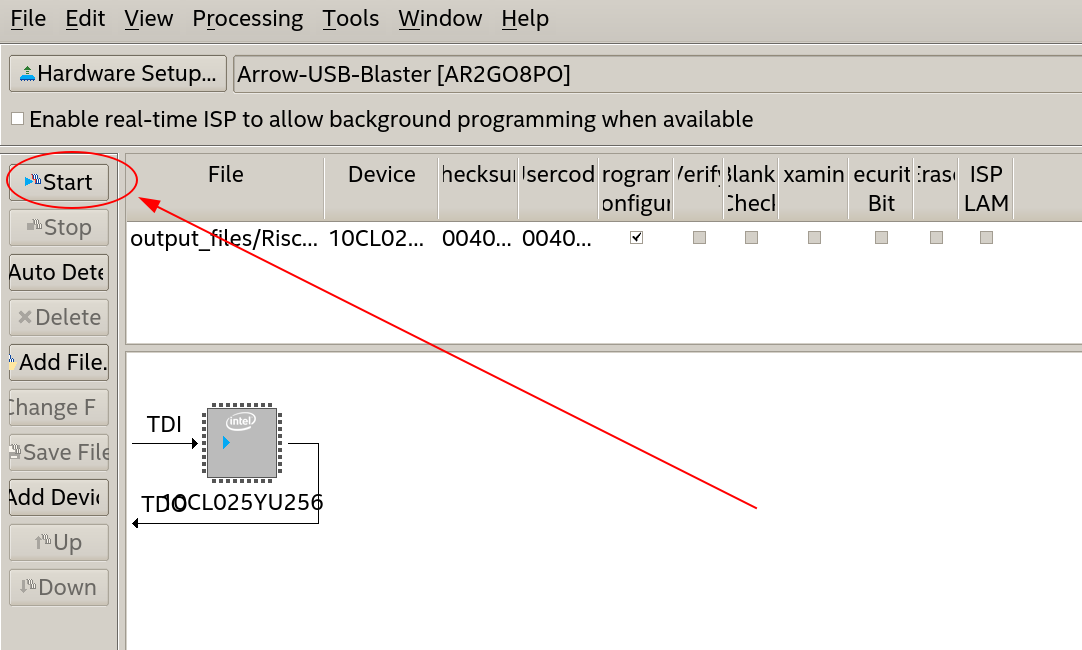
\includegraphics[scale=0.6]{img/quartus_programmer_start.png}
        \caption{Starten des Flashens des FPGAs}
        \label{fig:quartus_programmer_start}
    \end{figure}


    \section{Kompilieren des Programmcodes}
    \section{Flashen des Mikrocontrollers}

